\chapter{L'apprentissage supervisé avec les réseaux de neurones convolutionnels}

\section{Introduction}

Après la construction de notre base de données qui contient les images avec
les distances respectives, nous pouvons entamer la création du modèle qui
permettra l'estimation de distances à partir d'images en appliquant un
apprentissage supervisé sur les données. Nous proposons donc notre propre
architecture d'un réseau de neurones convolutionnel.

Nous commençons par la description de la structure de nos
données et les prétraitements appliqués sur ces données. Ensuite, nous présentons
les réseaux convolutionnels que nous avons conçus pour effectuer l'apprentissage
selon notre approche.
Par la suite, nous exposons notre méthode d'apprentissage et les paramètres
que nous avons choisis pour le réaliser.

\section{Les données et les prétraitements}

Nous avons pris des données à partir de plusieurs sources pour construire des
ensembles de données. Chaque ensemble contient un nombre considérable d'images et
de distances dont chaque image correspond à un nombre de distances ($3$ distances
pour chacune). Les images représentent les entrées du modèle et les distances
représentent les sorties.

\subsection{Les distances}

Pour simplifier l'apprentissage, nous avons besoin de réduire le nombre de
distances prises à une seule distance par image. Cette opération doit être faite
à l'aide d'une fonction mathématique. Nous avons choisi d'appliquer la
\emph{médiane} après avoir éliminé les distances inconnues.

Par exemple, si on suppose qu'une image correspond aux distances $1.24$, $1.21$, $1.25$, la
distance choisie est $1.24$ car $1.21 < 1.24 < 1.25$. Par contre, si nous avons
les valeurs $0.95$, $9.99$, $0.89$, la distance choisie est $(0.95+0.89)/2 = 0.92$
car $9.99$ est une valeur numérique dont on considère qu'elle signifie que la distance est inconnue.
Elle sera remplacée par la valeur spéciale $NaN$\footnote{\keyword{Not a Number:
constante qui indique que la donnée n'a pas une valeur numérique valide.}}.
Dans ce cas, la médiane est équivalente à la moyenne.
De même, si nous avons seulement une seule distance connue, par exemple :
$9.99$, $9.99$, $0.67$, le résultat est cette valeur. Dans certaines instances,
il se peut que toutes les valeurs soient invalides, dans ce cas, nous somme obligés
de considérer la distance comme inconnue. La distance trouvée après ce traitement
est transformée en un vecteur binaire de $4$ cases où pour chaque distance il
y a une case mise à $1$ et les autres à $0$. Ce traitement permet de passer d'
un problème de régression à un problème de classification en distribuant
les distances comme il est indiqué dans le tableau suivant.

\begin{table}[h]
  \centering
  \begin{tabular}{|l|c|c|c|c|}
    \hline
    Classe & Petite & Moyenne & Grande & Inconnue \\
    \hline
    Intervalle & $[0,1.5[$ & $[1.5,3[$ & $[3,4.5[$ & $[4.5,+\infty[$ \\
    \hline
  \end{tabular}
  \caption{La distribution des distances (en mètres) sur les classes}
\end{table}

Par exemple, une distance de $1.75m$ appartient aux distances moyennes
selon le tableau, donc elle sera représentée par un vecteur $x$ de $4$ cases
où la deuxième contient la valeur $1$ et les autres contiennent $0$. Formellement,
nous représentons cela par la notation mathématique suivante.

$$ x =
\begin{pmatrix}
  0\\
  1\\
  0\\
  0\\
\end{pmatrix}
$$

Les distances inconnues sont représentées par la valeur constante $9.99$ et donc
appartiennent évidemment à la dernière classe.

\subsection{Les images}

Les images stockées ont une taille de $96 \times 96$ pixels et contiennent $3$
canaux dont chacun contient les valeurs d'une couleur parmi le rouge, le vert et
le bleu. Elles sont transformées au moment du chargement en images de niveaux
de gris qui n’ont qu’un seul canal. En même temps, elles sont réduites par un
facteur de $\frac{1}{2}$, ce qui donne des images de taille $48 \times 48$.
Ces petits prétraitements ont été effectuées afin de réduire la taille de données
fournies pour l'apprentissage, ce qui permet de l'accélérer significativement.

\begin{figure}[h]
\begin{center}
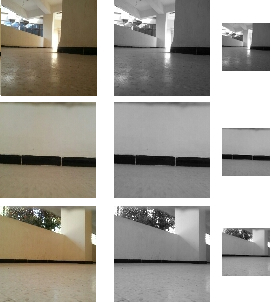
\includegraphics[width=0.4\textwidth]{Image-transformation}
\caption{Les prétraitements appliqués sur les images}
\end{center}
\end{figure}

\subsection{La transformation de données}

Afin d'alimenter nos modèles d'apprentissage, nous devons transformer l'ensemble
d'images et de distances en matrices multidimensionnelles portant les mêmes
informations. Les distances sont représentées par une matrice de deux dimensions :
la première pour les instances de distances dans un sous-ensemble, et l'autre pour
les classes d'une instance (dans notre cas il y a $4$). Par ailleurs, les images
sont représentées par une matrice de quatre dimensions dont la première correspond
aux instances, les deux suivantes à la hauteur et à la largeur
respectivement ($48$ pour les deux dans notre cas). La dernière représente le
nombre de canaux dans l'image ($1$ pour les images en niveaux de gris).

\section{Le modèle d'apprentissage}

Nous avons proposé deux architectures de réseaux de neurones convolutionnels composées
de plusieurs couches séquentielles de différents types. Ces architectures
séquentielles relativement profondes ont une structure inspirée de celle du
réseau \keyword{VGGNet} \cite{simonyan2014very}. La différence entre les deux
réside dans la profondeur et les hyperparamètres de chacune d'elles.

\begin{figure}[h]
\begin{center}
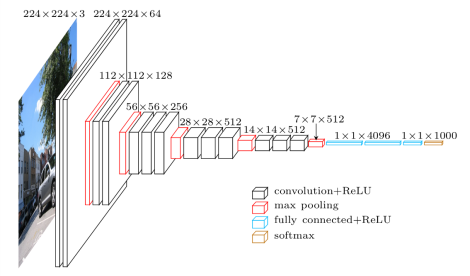
\includegraphics[width=0.5\textwidth]{imagenet_vgg16}
\caption{L'architecture de la variante du réseau VGGNet qui a 16 couches \cite{blier2016abrief}}
\end{center}
\end{figure}

\subsection{La description}

Les architectures sont composéss de grandes parties. Les premières sont
constituées de deux couches convolutionnelles suivies par une couche de regroupement,
tandis que la dernière est composée uniquement d'une couche dense. La
profondeur d'une couche convolutionnelle augmente d'une partie à une autre
bien que la taille spatiale de leur filtre diminue.

Le choix des couches convolutionnelles vient du fait qu'elles sont les plus
adaptées aux applications de la reconnaissance d'images car elles prennent en
considération la structure multidimensionnelle de l'image. De plus, vue que
chaque neurone de ces couches est connecté à un sous-ensemble de neurones de la
couche précédente, les paramètres dont le réseau doit apprendre sont moins nombreux et cela
est dû au \keyword{partage des paramètres}. Les sorties $z$ de chaque couche
convolutionnelle sont filtrées par la fonction d'activation ReLU (Rectified Linear Unit)
qui a la formule suivante.

$$
\mathrm{ReLU}(z) = \max(0,z) \cite{NIPS2012_4824}.
$$

Une couche de regroupement par le maximum est insérée après chaque ensemble de couches
convolutionnelles. Ce type permet de réduire la taille de l'image en appliquant
la fonction mathématique $\max$ sur les pixels adjacents dans chaque région. Cette
opération permet de réduire la variance intraclasse en diminuant les informations
inutiles. Pour chaque matrice de deux dimensions $A(N \times M)$, le regroupement
par le maximum $\mathrm{MaxPool}$ est défini par la formule suivante.

$$
\mathrm{MaxPool}(A) = \max(\{A_{n,m} | 1 \leq n \leq N, 1 \leq m \leq M\}) \cite{scherer2010evaluation}.
$$

Dans le dernier niveau du réseau, une couche dense est insérée afin de
rassembler tous les caractéristiques détectées à travers toute l'image, car cette
dernière contient des caractéristiques différents d'une région à une autre.
La couche de sortie est aussi une couche dense dont le nombre de perceptrons est
égale au nombre de classes (dans notre cas, c'est $4$). Les résultats $z$ sont
transmis vers la fonction $\mathrm{Softmax}$ afin de les normaliser pour
qu'ils représentent la probabilité dans l'intervalle $[0-1]$ de chaque classe.
Cette fonction est décrite par la formule suivante.

$$
\mathrm{Softmax}(z) = \frac{\mathrm{e}^{z_j}}{\sum^K_{k=1}\mathrm{e}^{z_k}}~\forall{j=\overline{1,K}} \cite{bridle1990probabilistic}.
$$

La raison pour laquelle l'architecture séquentielle est choisie est que les
couches peu profondes détectent
les caractéristiques de bas niveau (par exemple les lignes et les contours). Elles
ne sont pas nombreuses généralement, contrairement aux couches profondes qui détectent
les caractéristiques de haut niveau (comme les formes et les objets).
Cela est possible car la zone de couverture d'un neurone
augmente en parallèle avec sa profondeur.\cite{michael2015neural,Goodfellow-et-al-2016}

\subsection{La représentation textuelle}

L'architecture du réseau est sauvegardée comme un fichier texte sous le format
JSON (JavaScript Object Notation) \cite{introducing2012ecma}.
L'utilisation de ce type de fichier
permet de la créer, la copier et la modifier sans rien changer dans le
programme responsable de la construction du réseau. Elle est représentée comme un objet
ayant plusieurs attributs et leur valeur enregistrées dans un ordre précis.
Les attributs représentent les noms de couches et les valeurs contiennent
leur description. Chaque valeur est un objet contenant lui-même d'autres attributs
et d'autres valeurs dépendant du type de la couche décrite.

Les couches convolutionnelles ont quatre attributs :

\begin{itemize}
  \item \texttt{field\_size} : une valeur numérique entière strictement positive
  représentant la dimension horizontale et verticale du filtre de la convolution,
  \item \texttt{stride\_size} : une valeur numérique entière strictement positive
  représentant le pas de déplacement du filtre,
  \item \texttt{padding} : une des deux valeurs : \texttt{SAME} qui signifie
  l'utilisation de rembourrage par zéros, et \texttt{VALID} qui signifie le cas
  contraire,
  \item \texttt{depth} : une valeur numérique entière strictement positive représentant
  la profondeur de la couche, autrement dit, le nombre de matrices de paramètres
  partagées.
\end{itemize}

Les couches de regroupement par le maximum ont seulement les attributs \texttt{field\_size},
\texttt{stride\_size} et \texttt{padding} qui ont les mêmes sens. Les couches denses
n'ont que l'attribut \texttt{depth} qui dénote le nombre de perceptrons.

\subsection{La première architecture}

La première partie du réseau est constituée de deux couches convolutionnelles
ayant une profondeur égale à $16$ et dont la taille du filtre de chacune est
$5 \times 5$ déplacé par une unité à la fois, horizontalement et verticalement,
en ajoutant un rembourrage par zéros sur les quatre bords. Cela permet de garder
les dimensions originales de l'image entrante.
Elles sont suivies par une couche de regroupement par le maximum ayant un filtre
de taille $2 \times 2$ et un déplacement de $2$, ce qui réduit les dimensions de
l'entrée par un facteur de $\frac{1}{2}$. La deuxième partie est
identique à la première sauf que la profondeur de chaque couche convolutionnelle
est de $32$ et la taille du filtre de la convolution devient $3 \times 3$. Dans la
troisième partie, la couche dense contient $64$ perceptrons et elle est reliée
à toutes les sorties de la couche précédente. La couche de sortie est un
vecteur de taille $4$ où chaque perceptron représente une classe.

La figure suivante présente cette architecture. Les rectangles verts représentent
les couches convolutionnelles, les bleus représentent les couches de regroupement,
et les rouges représentent les couches denses.

\begin{figure}[h]
  \centering
  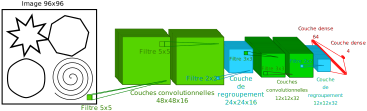
\includegraphics[width=\textwidth]{CNN1}
  \caption{Une représentation graphique de la première architecture}
\end{figure}

Le contenu du fichier qui décrit cette architecture est le suivant.
\lstinputlisting[caption=La représentation textuelle de la première architecture]
{../Code/PC/CNN-C5x16C5x16P2x2C3x32C3x32P2x2F64O4.json}

\subsection{La deuxième architecture}

Elle ressemble à la première mais elle est composée de quatre
parties principales. La première contient deux couches convolutionnelles ayant
un filtre de taille $7 \times 7$ et deux profondeurs de $8$ et $12$.
La deuxième contient des couches similaires dont le filtre a une taille de $5 \times 5$
et ses profondeurs sont de $16$ et de $24$. Les deux couches de la troisième parties ont
un filtre de taille $3 \times 3$ et des profondeurs de $32$ et $48$.
De même, une couche de regroupement est insérée après les deux couches
convolutionnelles dans les deux premières parties. Identiquement à l'architecture
précédente, celle-ci contient une couche dense de $64$ perceptrons dans la
dernière partie.

\begin{figure}[h]
  \centering
  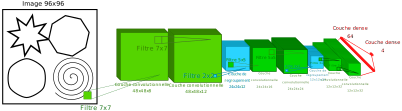
\includegraphics[width=\textwidth]{CNN2}
  \caption{Une représentation graphique de la deuxième architecture}
\end{figure}

\lstinputlisting[caption=La représentation textuelle de la deuxième architecture]
{../Code/PC/CNN-C7x8C7x12P2x2C5x16C5x24P2x2C3x32C3x48F64O4.json}

\section{L'apprentissage automatique du modèle}

Afin de rendre notre modèle opérationnel, nous devons changer ses paramètres en
appliquant un apprentissage supervisé par les données. En effet, nous devons
d'abord définir les modèles d'évaluation du réseau qui sont manipulés pour pouvoir
effectuer l’entraînement.

\subsection{La fonction de coût}

Les réseaux de neurones sont utilisés pour approximer des fonctions non linéaires.
Mais cette approximation n'est pratiquement jamais parfaite, il existe toujours
une quantité d'erreur entre les valeurs générées par le réseau et les valeurs réelles.
De ce fait, il faut définir une fonction permettant de calculer cette erreur et utiliser
une approche mathématique pour la minimiser.

Étant donné la transformation de ce problème vers une tâche de classification,
la formule d'erreur interclasses la plus adéquate est \keyword{l'entropie croisée}
qui est décrite par la formule :

$$
H(p, y) = -\sum_i y_i \cdot \log(p_i),
$$

avec $p$ le vecteur des valeurs calculées par le réseau et $y$ le vecteur des valeurs réelles.

Comme les valeurs de $y$ sont binaires, seulement la probabilité de l'élément de
la bonne classe qui sera prise en considération dans le calcul, et tous les autres
probabilités seront éliminées, et la somme de produits de logarithmes devient
juste un simple logarithme.
Par exemple, si nous avons comme données :

$$
y =
\begin{pmatrix}
  0\\
  1\\
  0\\
  0\\
\end{pmatrix}
~
\mathrm{et}
~
p =
\begin{pmatrix}
  0.6\\
  0.9\\
  0.3\\
  0.2\\
\end{pmatrix}
$$

la valeur de l'entropie croisée est calculée comme suit :

$$
H(p, y) = -(0 \times \log(0.6) + 1 \times \log(0.9) + 0 \times \log(0.3) + 0 \times \log(0.2))
$$
$$
H(p, y) = -\log(0.9) \approx 0.1054.
$$

\subsection{L'optimiseur}

L’apprentissage est effectué en minimisant la valeur d'erreur par une des fonctions
d'optimisation connus sous le nom d'\keyword{optimiseurs} qui sont basés sur la décente
du gradient. Cette dernière consiste à changer les poids du modèle dans les sens inverses
aux signes des dérivées partielles par un facteur nommé le \keyword{taux d'apprentissage}.
Il faut choisir et changer sa valeur avec précaution car une mauvaise valeur
risque d'empêcher l'optimiseur de converger vers l'optimum ou de gaspiller beaucoup
d'itérations pour ce faire.\cite{DBLP:journals/corr/Ruder16}

Dans ce travail, nous avons choisi l'optimiseur \keyword{Adadelta} \cite{DBLP:journals/corr/abs-1212-5701}
car il rend le choix du taux d'apprentissage sans aucune importance grâce à sa
formule de mise à jour de paramètres qu'elle les change indépendamment
selon la fréquence de modification de chacune à travers le temps.\cite{DBLP:journals/corr/Ruder16}

\subsection{L'exactitude}

Afin de pouvoir évaluer les performances d'un réseau de neurones, il faut définir
une formule d'exactitude permettant de calculer le nombre de résultats jugés
corrects par rapport au nombre total. La formule que nous avons utilisée est
la moyenne de comparaisons d'indices dont la valeur est maximale sur les
vecteurs de prédictions $P_i$ et les vecteurs d'étiquettes $Y_i$. Nous pouvons représenter
cela par la formule suivante.

$$
Acc = \frac{\sum_{i=1}^N(\mathrm{argmax}(P_i) = \mathrm{argmax}(Y_i))}{N},
$$

où $N$ est le nombre de vecteurs de prédictions dans l'ensemble et
$\mathrm{argmax}$ est la fonction qui donne l'indice de l'élément qui a la plus grande
valeur dans le vecteur numéro $i$.

\`A titre d'exemple, si nous avons les vecteurs de prédictions et les vecteurs
d'étiquettes suivants (représentés sous forme de matrices où les vecteurs sont transposés
et empilés sur la première dimension) :

$$
Y =
\begin{pmatrix}
  0 & \mathbf{1} & 0 & 0\\
  \mathbf{1} & 0 & 0 & 0\\
  0 & 0 & \mathbf{1} & 0\\
\end{pmatrix}
~
\mathrm{et}
~
P =
\begin{pmatrix}
  0.6 & \mathbf{0.9} & 0.3 & 0.2\\
  0.3 & 0.1 & \mathbf{0.7} & 0.5\\
  0.1 & 0.3 & \mathbf{0.5} & 0.1\\
\end{pmatrix},
$$

l'indice de l'élément ayant la valeur maximale sur chaque ligne dans les deux
matrices est le même pour les lignes $1$ et $3$, ce qui n'est pas vrai pour la
ligne $2$. L'exactitude dans ce cas est clairement égale à $\frac{2}{3} \approx 0.6667$
qui signifie que $66.67~\%$ de prédictions du réseau sont corrects.

\section{Conclusion}

Avant d'arriver à fixer la structure de nos données et choisir les différentes
architectures décrites dans ce chapitre, nous avons essayé plusieurs combinaisons
de variations de ces dernières que nous n'avons pas pu les mentionner.
Les tests que nous avons effectués ont montré les limitations de ces variations
en termes de complexité et vitesse d'exécution, et donc ils nous ont obligé de
transiter vers les modèles présentées ici.

Le prochain chapitre portera sur l'exécution de l'apprentissage automatique sur
ces modèles et ces structures en utilisant les ensembles de données que nous avons
collecté. Nous suivrons l'amélioration des performances du modèles et nous
enregistrerons les statistiques d'exécution obtenus en même temps.
